\section{Simulation}
\label{sec:simulation}


\section{Changes since Technical Proposal}
\subsection{Simulation}
\label{sec:simulation}
The simulation of the proton on fixed-target collisions is done in two steps, primary proton-proton or proton-neutron collisions are simulated using Pythia8, and the particles produced are transported through the experimental setup using Geant4. Some important sources of background muons are not generated by default in Geant4, like decays of light vector mesons to $\mu^+\mu^-$, $\gamma$-conversions to $\mu^+\mu^-$, positron annihilation to $\mu^+\mu^-$. These are all rare processes, but can potentially cause background in the detector due to not being diverted by the active muon shield because of high momentum or wrong charge of the muon. Their rate had been increased artificially in the simulation by a factor $100$ to simulate enough statistics to study these events in detail.

% add figure of muon leaving hadron absorber as function of p/pt, with different sources, or table

For the heavy quark production, a procedure had been put in place to simulate also charm and beauty hadron production by the products of the primary proton nucleon collision~\cite{cascade}. % myBiblio.bib
This increases the yield expectation compared to the prediction in the Technical Proposal by a factor of $2.6$($1.9$) for  $1$($3$) $GeV/c$ HNLs in the acceptance.

Simulated in total $65$ billion protons on target with an energy cut for transporting particles after the hadron absorber of $10$ GeV, and $1.8$ billion protons on target with an energy cut of $1$GeV. The samples produced with charm and beauty hadrons correspond to about $100$ billion protons on target.

\begin{figure}[h]
\centering
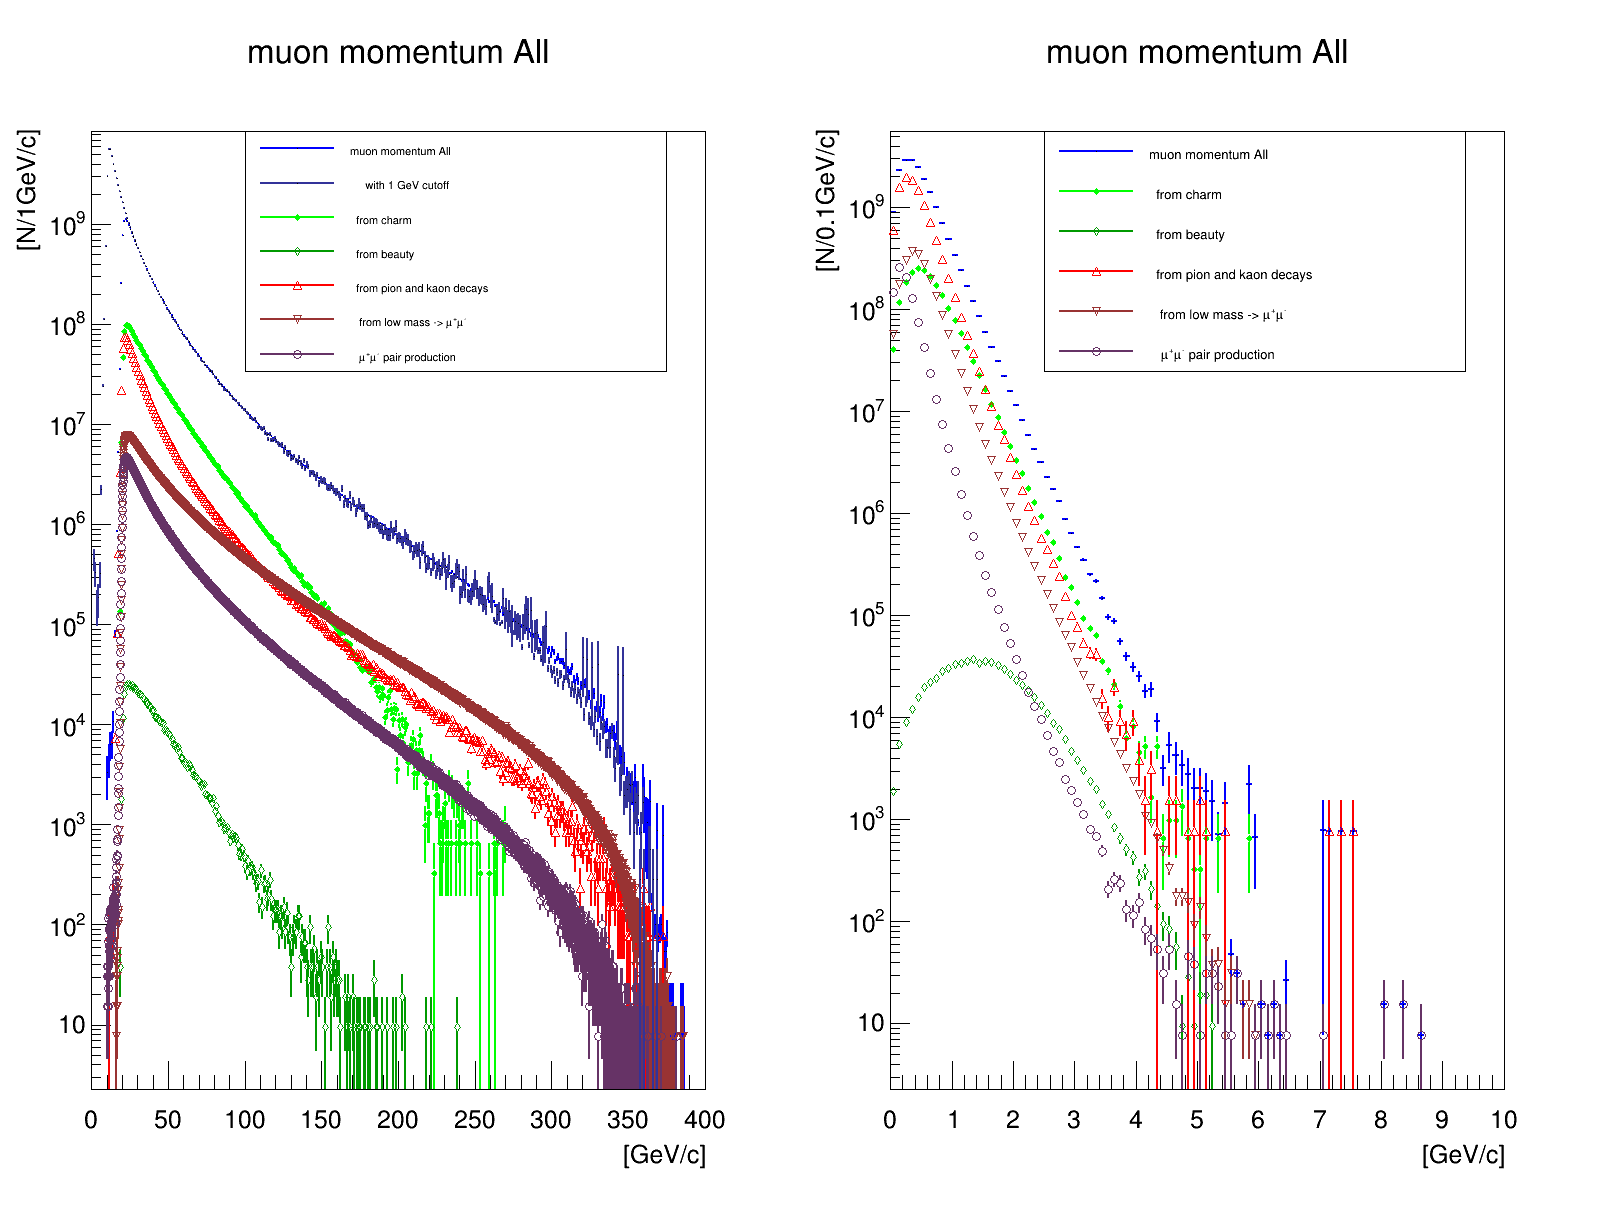
\includegraphics[width=8cm]{figs/muonMom.png}
\caption{Momentum distributions of muons leaving the hadron absorber, total momentum (left) and transverse momentum(right). Different contributions are shown. The rates are normalized to one spill ($5\times 10^{13} $) protons on target.}
\label{fig:muonMom}
\end{figure}

\begin{figure}[h]
\centering
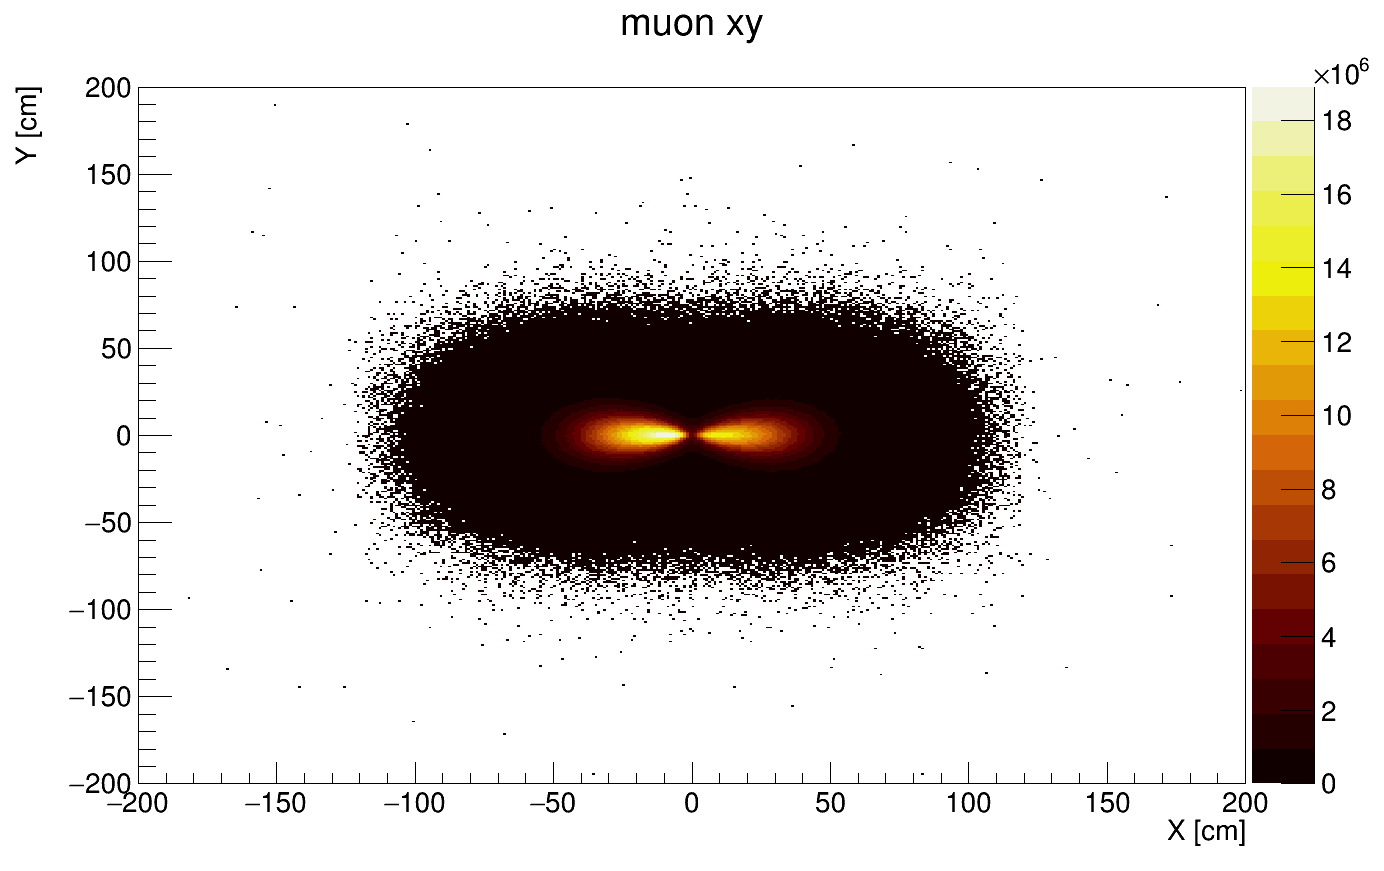
\includegraphics[width=8cm]{figs/muonXY.png}
\caption{Position of muons leaving the magnetized hadron absorber.}
\label{fig:muonXY.png}
\end{figure}


\begin{figure}[h]
\centering
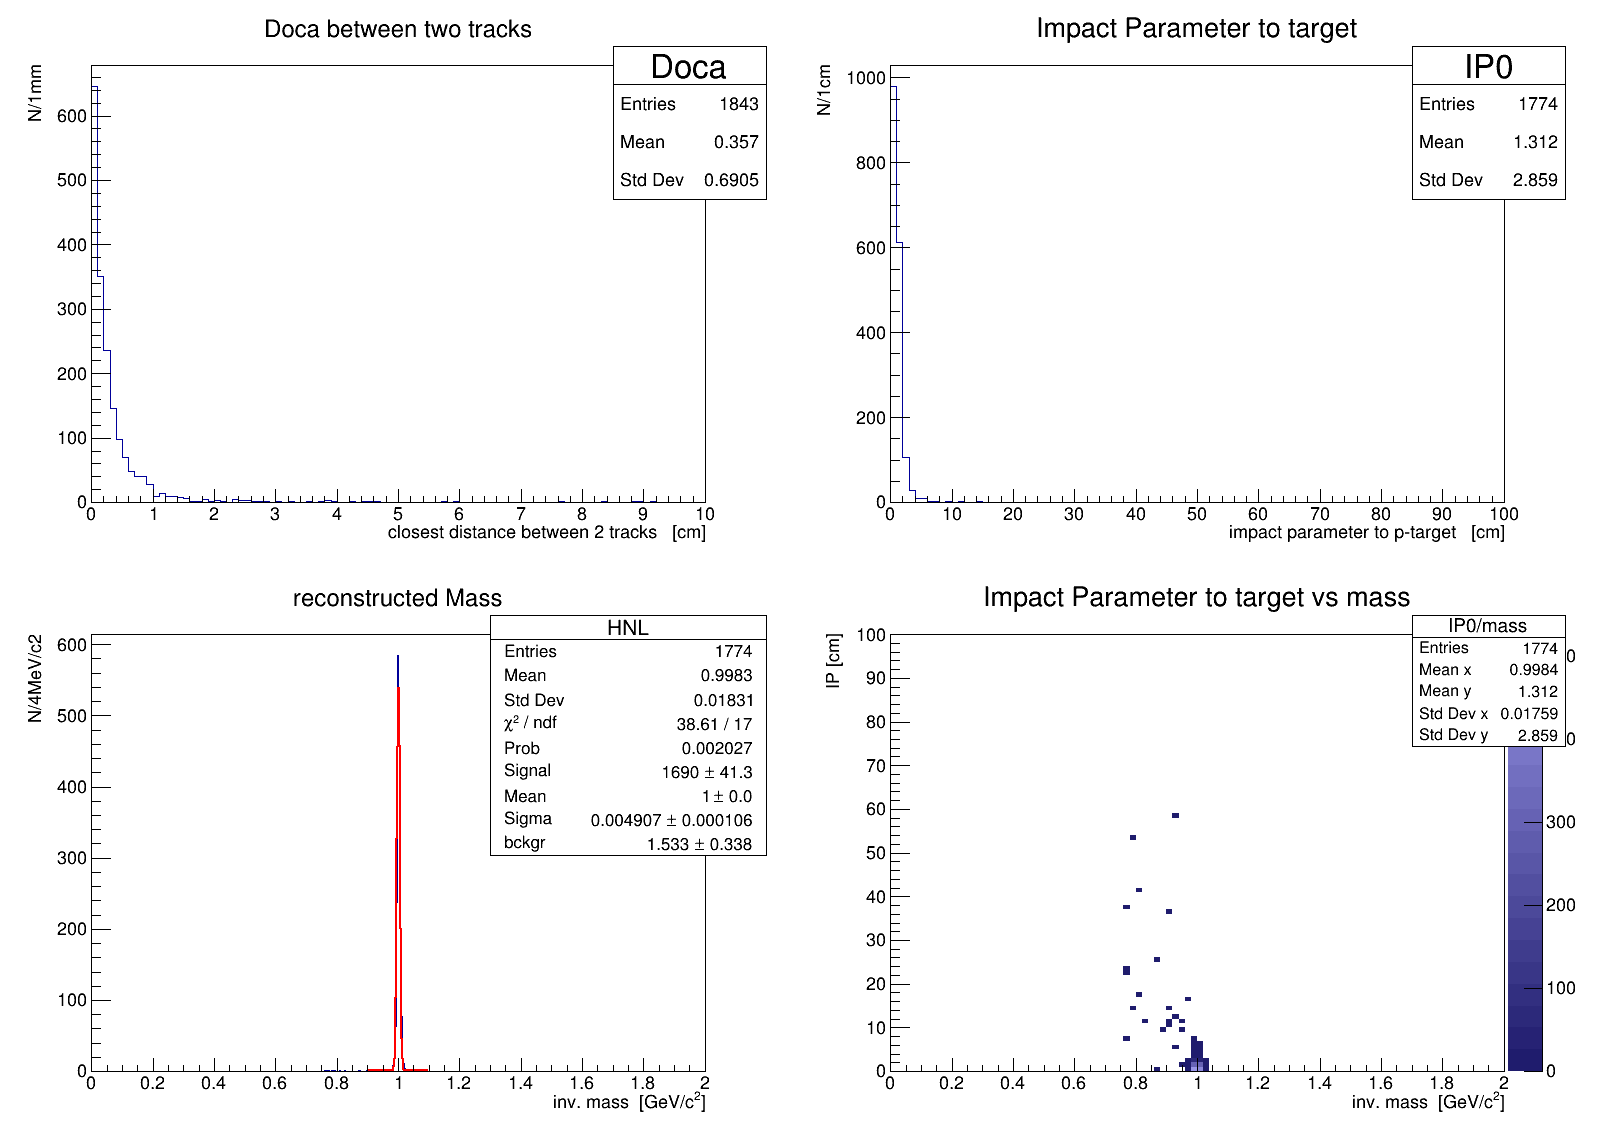
\includegraphics[width=8cm]{figs/mupiperformance.png}
\caption{Reconstruction of $HNL\rightarrow \mu^-\pi^+$.}
\label{fig:signalpimu.png}
\end{figure}

\begin{figure}[h]
\centering
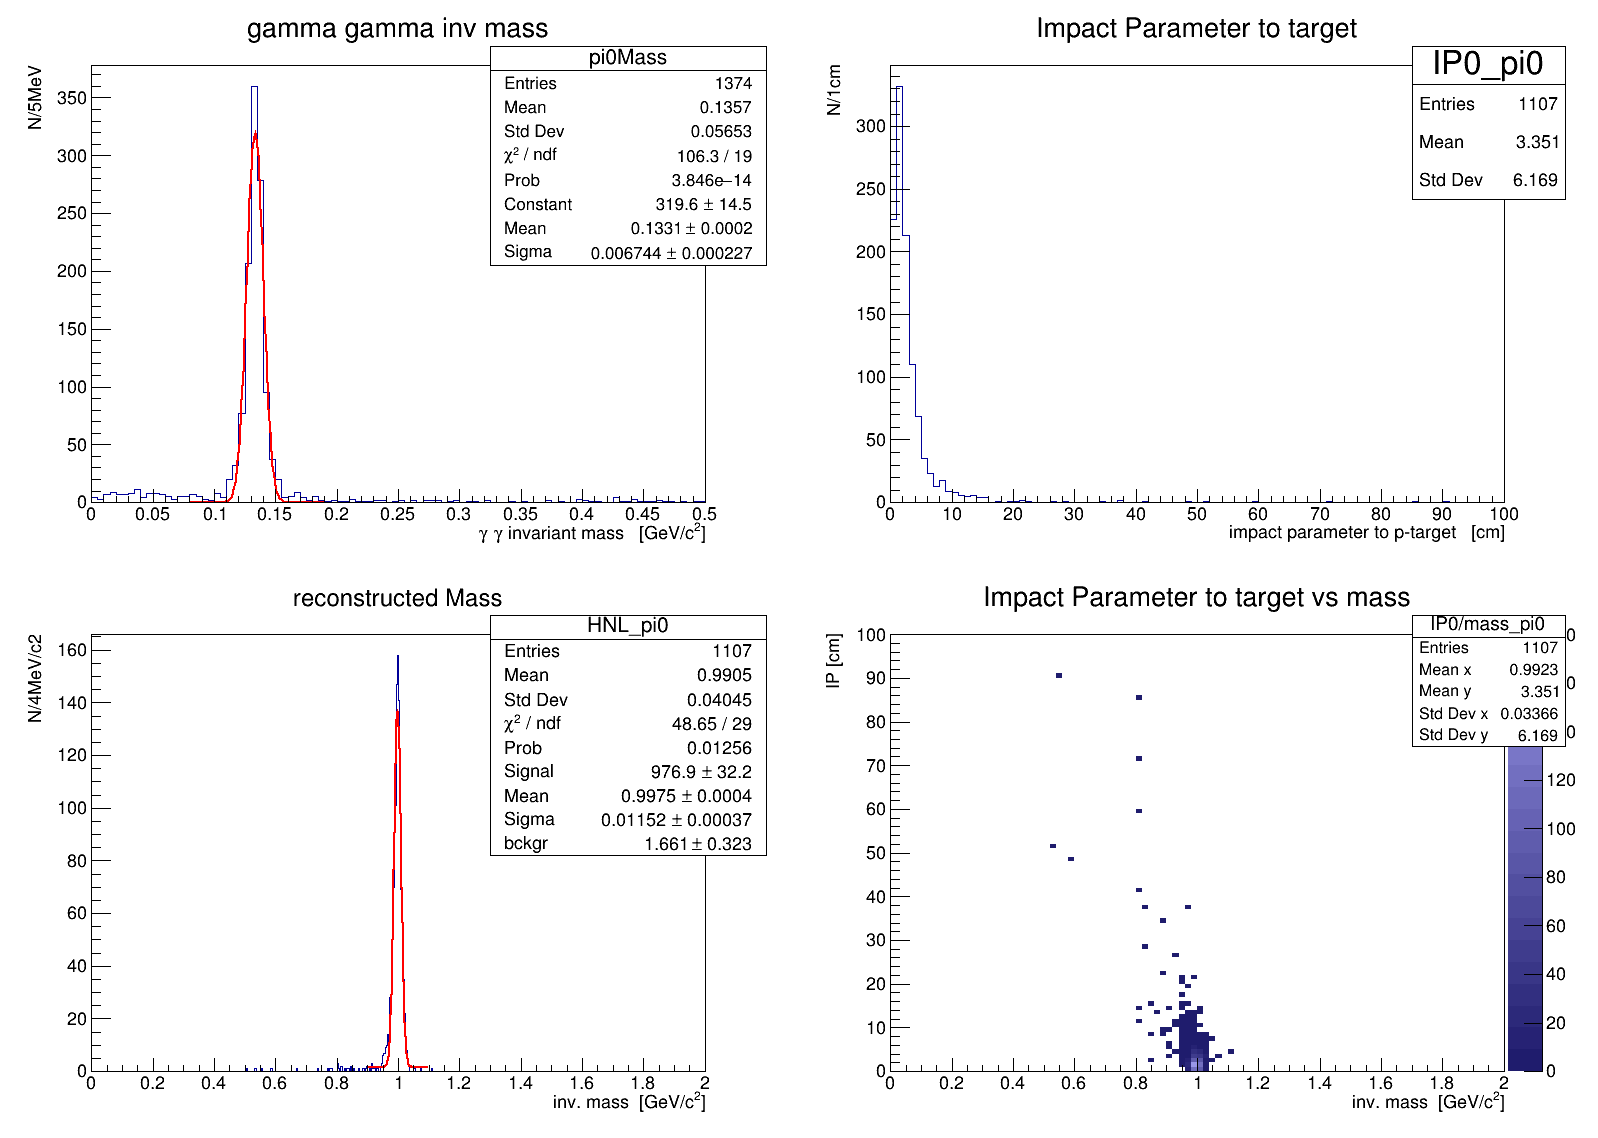
\includegraphics[width=8cm]{figs/murhoperformance.png}
\caption{Reconstruction of $HNL\rightarrow \mu^- \rho^+(\rightarrow\pi^+\pi^0(\rightarrow\gamma\gamma))$.}
\label{fig:signalrhomu.png}
\end{figure}

\begin{figure}[h]
\centering
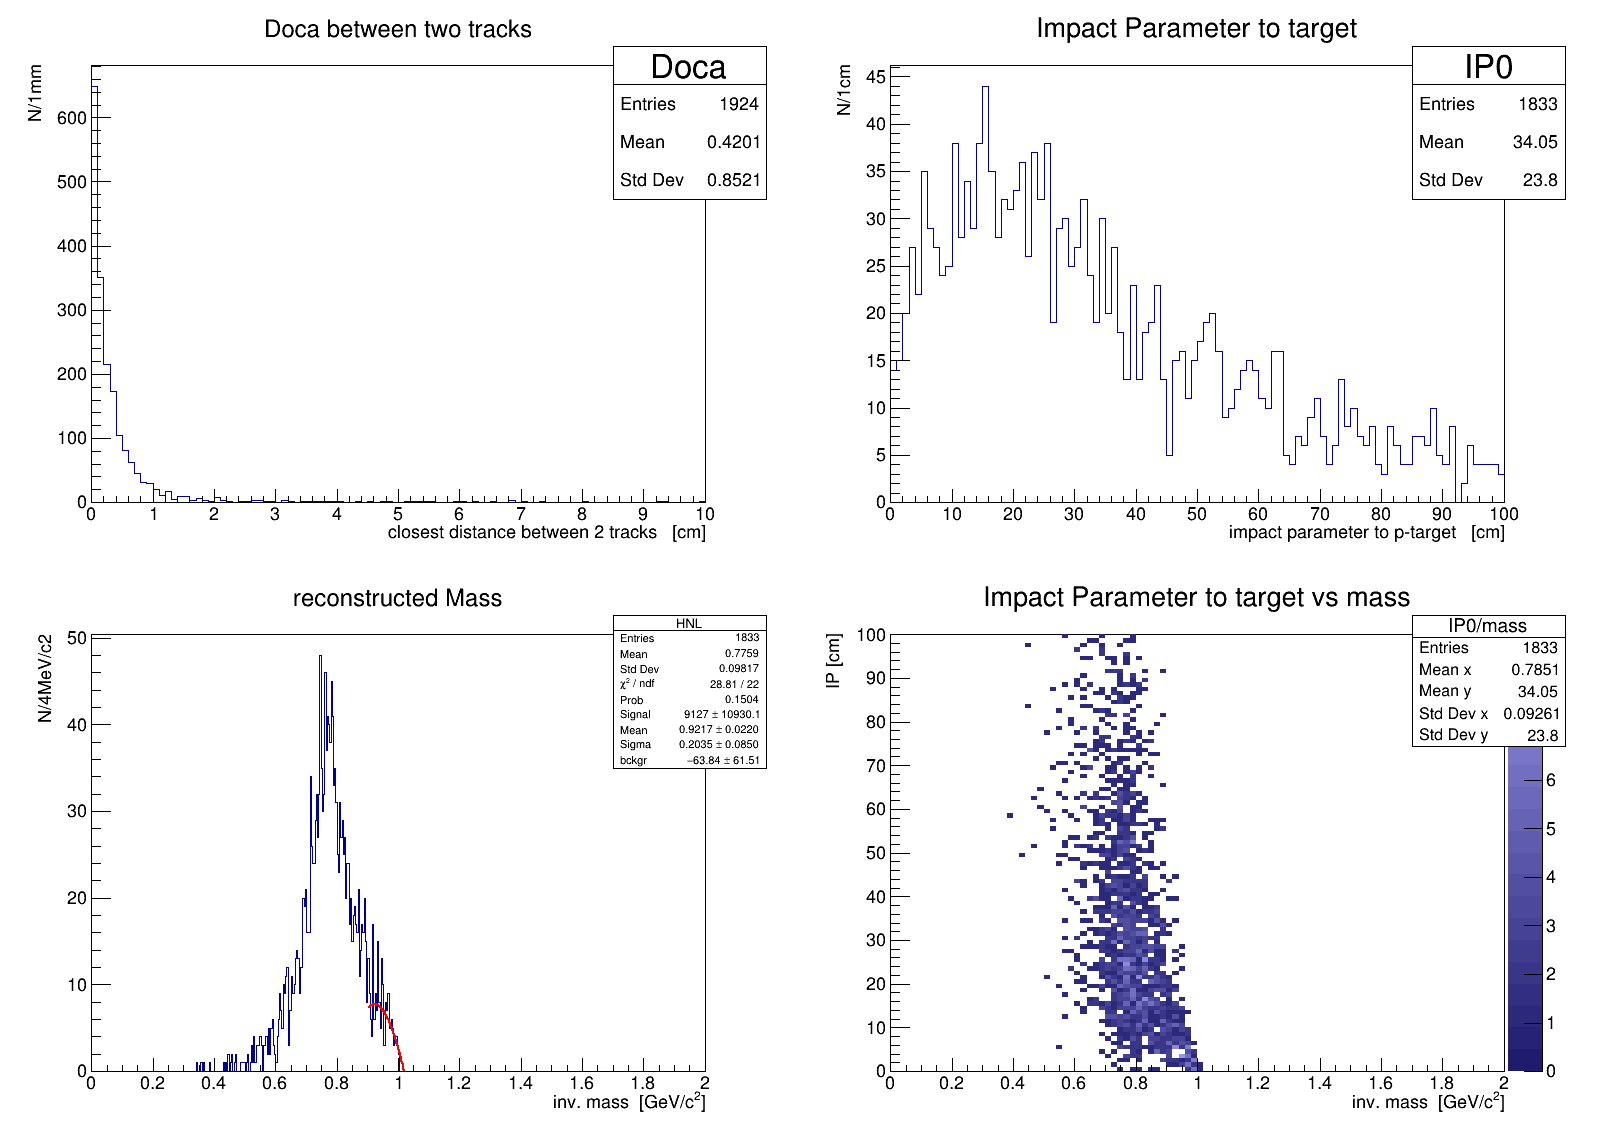
\includegraphics[width=8cm]{figs/numuperformance.png}
\caption{Reconstruction of $HNL\rightarrow \nu\rho^0(\rightarrow\pi^+\pi^-$.}
\label{fig:signalnumurho0.png}
\end{figure}

\begin{figure}[h]
\centering
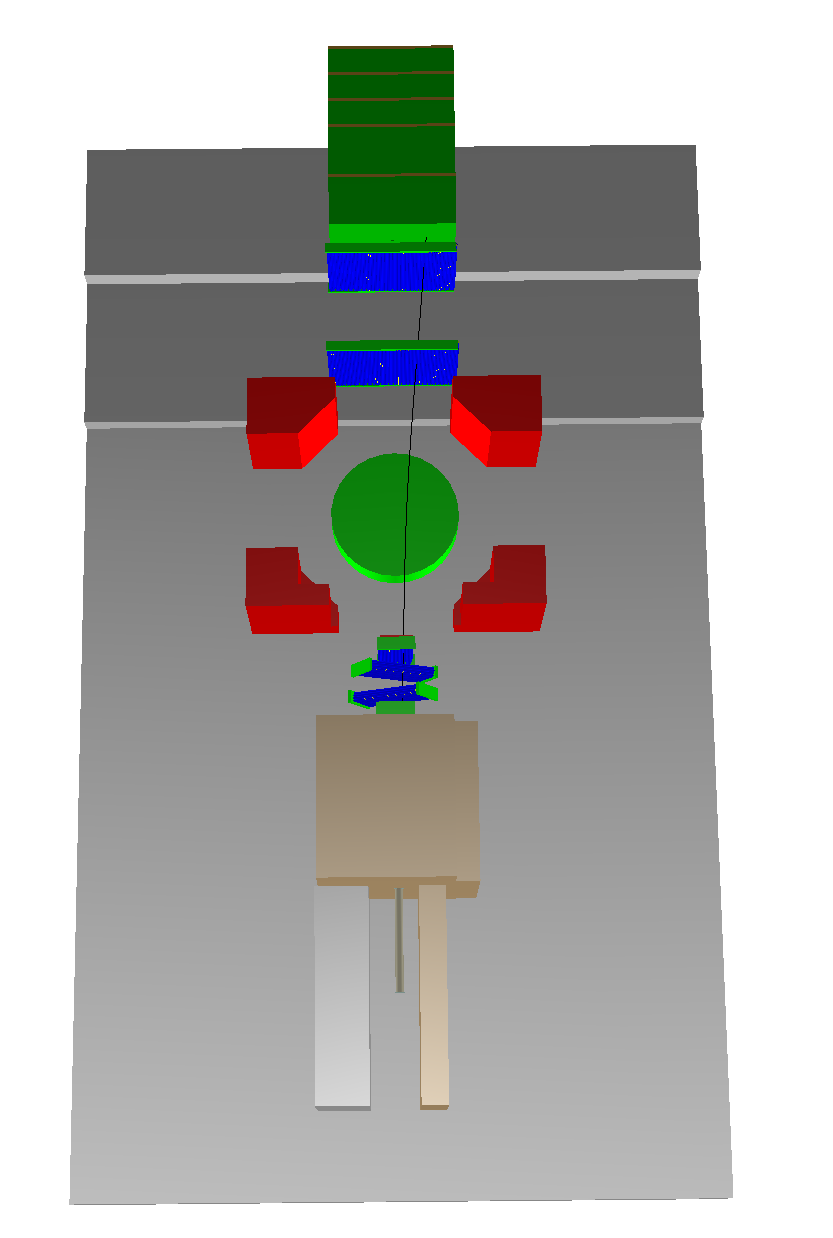
\includegraphics[width=8cm]{figs/muflux-setup-withTrack.png}
\caption{Muflux testbeam setup with a track reconstructed using FairShip. }
\label{fig:eventDisplay.png}
\end{figure}


Cross checks of simulation with data:
\begin{itemize}
  \item Studying Multiple Scattering with GEANT4 v10.3.2, The multiple scattering as implemented in the GEANT4 version currently employed in the FairShip simulation is compared to existing data and other models.
CERN-SHiP-NOTE-2017-003, see Fig.\ref{fig:data}. Good agreement is found.
  \item Comparing catastrophic energy loss of muons in a liquid krypton calorimeter (NA62, https://indico.in2p3.fr/event/420/contributions/29860/attachments/24033/29479/moriond.pdf ) with Geant4.  The Geant4 setup consists of $125$cm thick block of liquid krypton.
  Muons are shot on the block, and the energy deposited in the block is summed up.  (The muon critical energy for which radiative and ionization energy loss rates are equal is about $280$ GeV/c in liquid krypton and $350$ GeV/c for iron, D.E. Groom, N.V. Mokhov, and S.I. Striganov, “Muon stopping-power and range tables: 10 MeV–100 TeV,” Atomic Data and Nuclear Data Tables 78, 183–356 (2001).)  The mean energy deposited in the liquid krypton does not agree well with the mean energy loss expected for muons (right plot).
  \item A specific experiment had been setup in the CERN North Area to measure directly the rate and momentum of muons of $400$ protons impinging on a replica of the SHiP target after a $xx$m.
\end{itemize}


\begin{figure}[htb]
\begin{center}
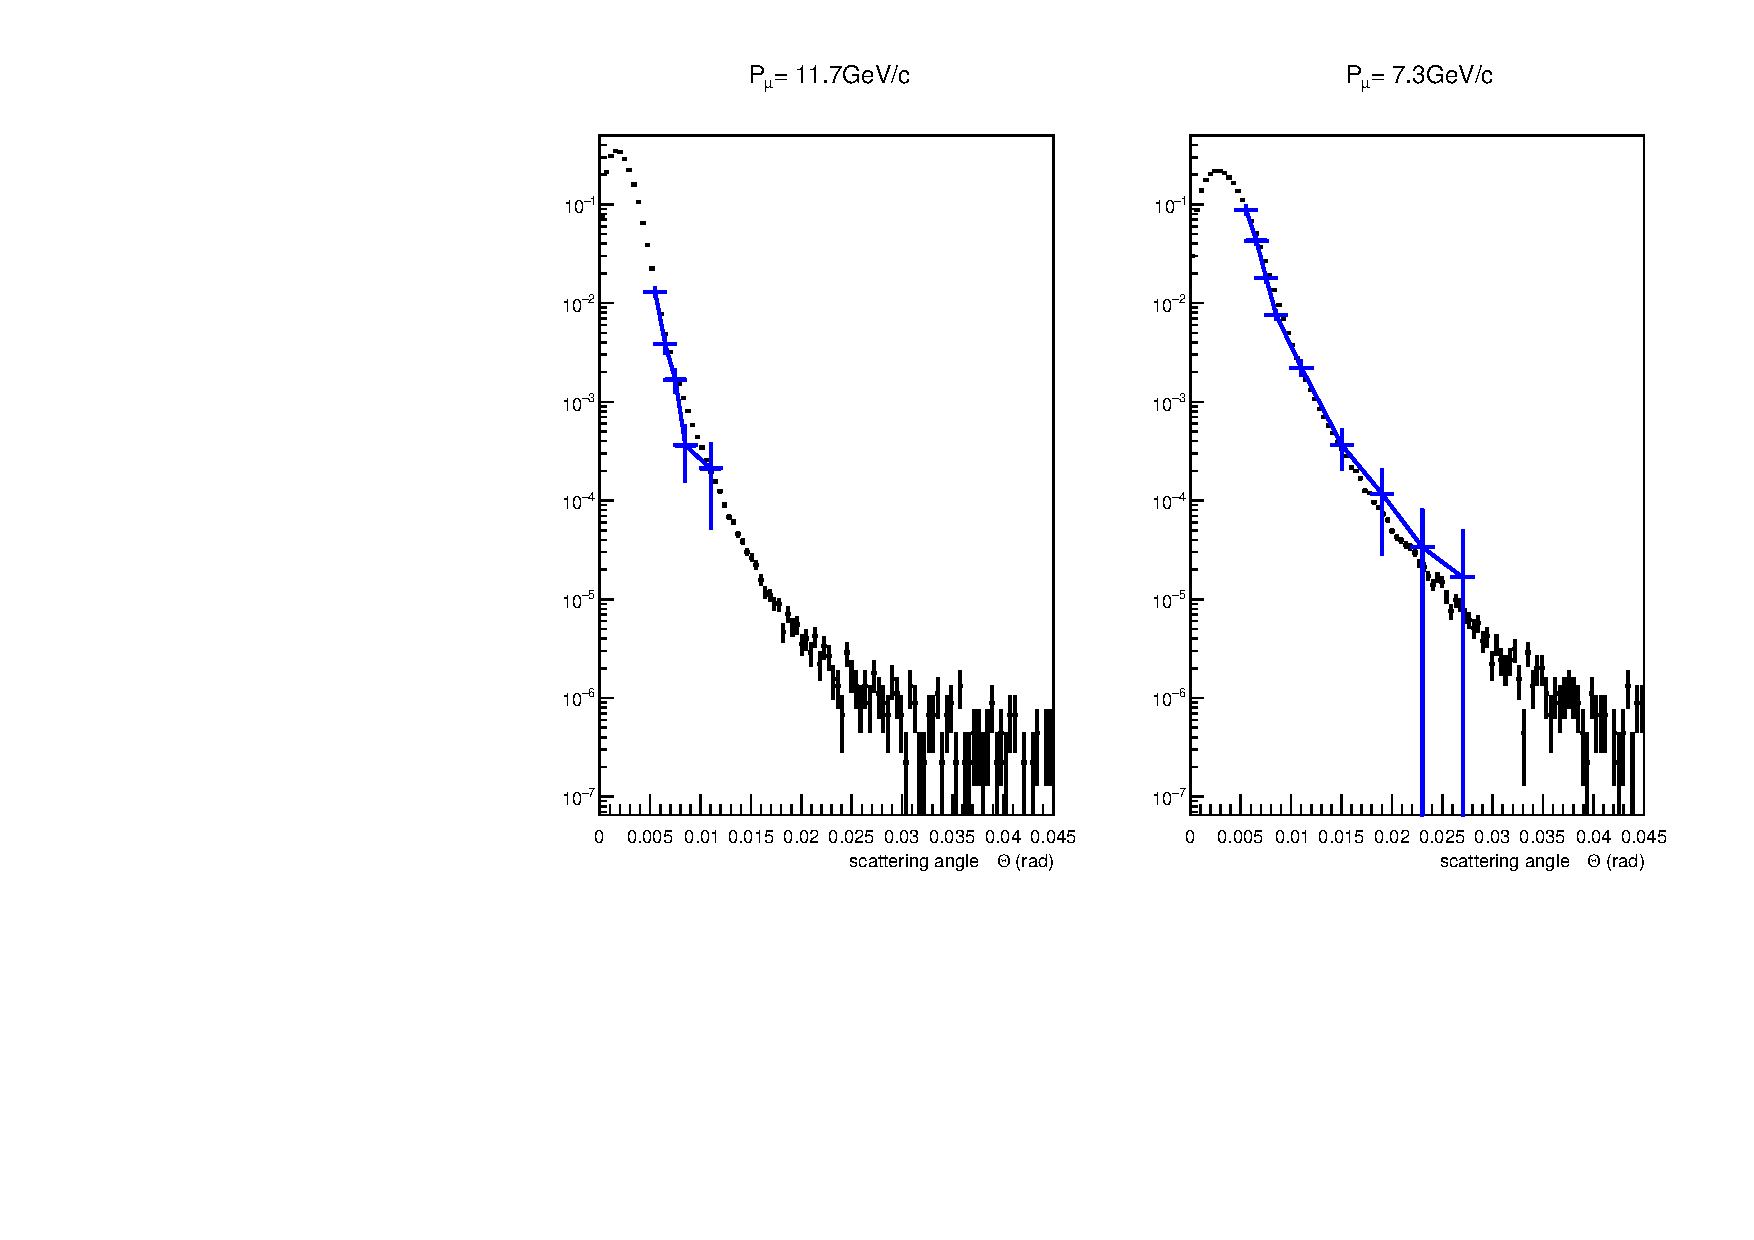
\includegraphics[width=0.8\linewidth]{figs/dataMSC.pdf}
\caption{ Comparison of the GEANT4 Monte Carlo simulation to the 11.7 GeV/c data-set (left) and 7.3 GeV/c data-set (right). Blue points are the measurements of \cite{Akimenko:1984qw}, black points are from the FairShip simulation. }
\label{fig:data}
\end{center}
\end{figure}

\begin{figure}[htb]
\begin{center}
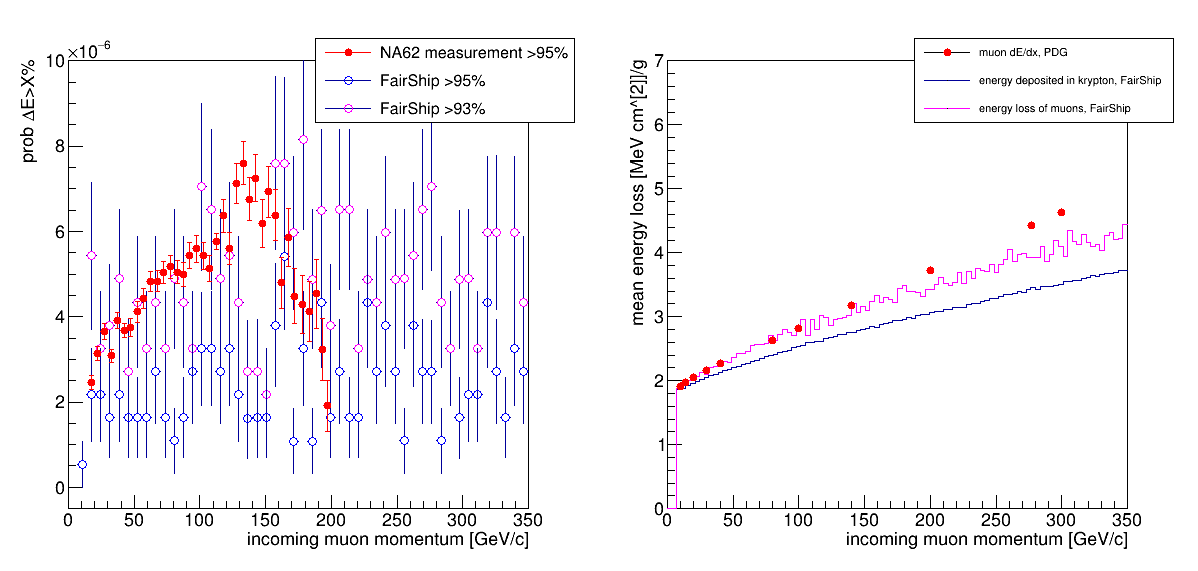
\includegraphics[width=0.8\linewidth]{figs/catastrophicEnergyLoss.png}
\caption{ Left: Probability that a muon releases in the liquid krypton calorimeter more than 95\% of its energy as a function of the muon momentum in GeV/c, red points NA62 measurements, blue points FairShip simulation, magenta points FairShip with >93\%.
Right: mean energy loss as function of muon momentum. Note, energy deposited in krypton is less than the energy loss of a muon. At higher energies, mean energy loss is lower than expected.}
\label{fig:data}
\end{center}
\end{figure}

\subsection{Detector Setup}
\label{sec:detectors}
Strawtracker diameter increased from $1$cm to $2$cm to save readout channels, no effect on momentum / vertex resolution observed.
Same dimensions for all straw tracker stations. Support material added to simulation.

Moved to use realistic field maps for the spectrometer magnet (from OPERA simulation) and for the active muon shield, compared to using an analytic function for the bending field (no return field) and constant fields in the active muon shield. The latter changed the background from ? to ? (ask Oliver,

Active muon shield optimized for frustum detector setup

many changes to nu tau detector, described elsewhere. Takes over in addition task of upstream veto tagger.

straw veto tagger removed, vertex information enough to veto background of $K_S$ decays.

added second Ecal detector option, splitCal, which is under study. Removed HCal



\subsection{Reconstruction}
\label{sec:reconstruction}
different pattern recognition algorithm tested. Reconstruction of signal decays to two charged tracks and a pi0.



